% This file was created with tikzplotlib v0.10.1.
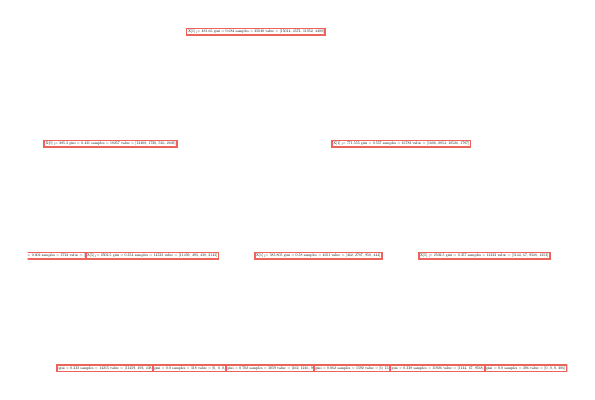
\begin{tikzpicture}

\definecolor{darkgray176}{RGB}{176,176,176}
\definecolor{tomato2369992}{RGB}{236,99,92}

\begin{axis}[
hide x axis,
hide y axis,
tick align=outside,
tick pos=left,
x grid style={darkgray176},
xmin=0, xmax=1,
xtick style={color=black},
y grid style={darkgray176},
ymin=0, ymax=1,
ytick style={color=black}
]
\draw (axis cs:0.153846153846154,0.125) node[
  scale=0.140017493769907,
  fill=white,
  draw=tomato2369992,
  line width=0.6pt,
  inner sep=3.6pt,
  text=black,
  rotate=0.0,
  align=center
]{gini = 0.332
samples = 14215
value = [11459, 493, 438, 1825]};
\draw (axis cs:0.307692307692308,0.125) node[
  scale=0.140017493769907,
  fill=white,
  draw=tomato2369992,
  line width=0.6pt,
  inner sep=3.6pt,
  text=black,
  rotate=0.0,
  align=center
]{gini = 0.0
samples = 318
value = [0, 0, 0, 318]};
\draw (axis cs:0.461538461538462,0.125) node[
  scale=0.140017493769907,
  fill=white,
  draw=tomato2369992,
  line width=0.6pt,
  inner sep=3.6pt,
  text=black,
  rotate=0.0,
  align=center
]{gini = 0.702
samples = 3059
value = [462, 1246, 907, 444]};
\draw (axis cs:0.615384615384615,0.125) node[
  scale=0.140017493769907,
  fill=white,
  draw=tomato2369992,
  line width=0.6pt,
  inner sep=3.6pt,
  text=black,
  rotate=0.0,
  align=center
]{gini = 0.062
samples = 1592
value = [0, 1541, 51, 0]};
\draw (axis cs:0.769230769230769,0.125) node[
  scale=0.140017493769907,
  fill=white,
  draw=tomato2369992,
  line width=0.6pt,
  inner sep=3.6pt,
  text=black,
  rotate=0.0,
  align=center
]{gini = 0.338
samples = 11926
value = [1144, 67, 9568, 1147]};
\draw (axis cs:0.923076923076923,0.125) node[
  scale=0.140017493769907,
  fill=white,
  draw=tomato2369992,
  line width=0.6pt,
  inner sep=3.6pt,
  text=black,
  rotate=0.0,
  align=center
]{gini = 0.0
samples = 206
value = [0, 0, 0, 206]};
\draw (axis cs:0.0769230769230769,0.375) node[
  scale=0.140017493769907,
  fill=white,
  draw=tomato2369992,
  line width=0.6pt,
  inner sep=3.6pt,
  text=black,
  rotate=0.0,
  align=center
]{gini = 0.602
samples = 3724
value = [1949, 1227, 88, 460]};
\draw (axis cs:0.230769230769231,0.375) node[
  scale=0.140017493769907,
  fill=white,
  draw=tomato2369992,
  line width=0.6pt,
  inner sep=3.6pt,
  text=black,
  rotate=0.0,
  align=center
]{X[5] <= 2502.5
gini = 0.354
samples = 14533
value = [11459, 493, 438, 2143]};
\draw (axis cs:0.538461538461538,0.375) node[
  scale=0.140017493769907,
  fill=white,
  draw=tomato2369992,
  line width=0.6pt,
  inner sep=3.6pt,
  text=black,
  rotate=0.0,
  align=center
]{X[1] <= 583.805
gini = 0.58
samples = 4651
value = [462, 2787, 958, 444]};
\draw (axis cs:0.846153846153846,0.375) node[
  scale=0.140017493769907,
  fill=white,
  draw=tomato2369992,
  line width=0.6pt,
  inner sep=3.6pt,
  text=black,
  rotate=0.0,
  align=center
]{X[5] <= 2502.5
gini = 0.357
samples = 12132
value = [1144, 67, 9568, 1353]};
\draw (axis cs:0.153846153846154,0.625) node[
  scale=0.140017493769907,
  fill=white,
  draw=tomato2369992,
  line width=0.6pt,
  inner sep=3.6pt,
  text=black,
  rotate=0.0,
  align=center
]{X[0] <= 285.3
gini = 0.431
samples = 18257
value = [13408, 1720, 526, 2603]};
\draw (axis cs:0.692307692307692,0.625) node[
  scale=0.140017493769907,
  fill=white,
  draw=tomato2369992,
  line width=0.6pt,
  inner sep=3.6pt,
  text=black,
  rotate=0.0,
  align=center
]{X[1] <= 771.555
gini = 0.557
samples = 16783
value = [1606, 2854, 10526, 1797]};
\draw (axis cs:0.423076923076923,0.875) node[
  scale=0.140017493769907,
  fill=white,
  draw=tomato2369992,
  line width=0.6pt,
  inner sep=3.6pt,
  text=black,
  rotate=0.0,
  align=center
]{X[1] <= 481.66
gini = 0.684
samples = 35040
value = [15014, 4574, 11052, 4400]};
\end{axis}

\end{tikzpicture}
